\subsubsection{Mô tả các thực thể và Các thành phần}

\begin{itemize}
    \item \textbf{Nhóm Thiết bị người dùng cuối:}
    \begin{itemize}
        \item \textbf{User Device (Mobile/PC):} Thiết bị của người học, cán bộ hoặc khách vãng lai. Chạy trình duyệt web để tải thành phần \texttt{Frontend Application (ReactJS)}. Giao tiếp với hệ thống qua giao thức HTTPS.
        \item \textbf{Electronic Signage (Bảng LED chỉ dẫn):} Màn hình hiển thị tại các nút giao và cổng bãi xe. Nhận dữ liệu trạng thái bãi đỗ thời gian thực thông qua kết nối \texttt{WebSocket}.
    \end{itemize}

    \item \textbf{Nhóm Thiết bị IoT \& Phần cứng bãi xe:}
    \begin{itemize}
        \item \textbf{IoT Sensor Node:} Các cảm biến tại từng vị trí đỗ xe. Chạy firmware \texttt{PubSubClient} để phát hiện trạng thái (có/trống xe) và gửi tín hiệu qua sóng Wi-Fi.
        \item \textbf{IoT Gateway:} Thiết bị thu thập dữ liệu cục bộ từ nhiều cảm biến. Đóng gói dữ liệu và truyền về trung tâm thông qua giao thức \texttt{MQTT}.
        \item \textbf{Smart Gate:} Tích hợp đầu đọc thẻ từ (RFID/NFC) và máy phát vé tạm. Gửi yêu cầu xác thực thẻ và nhận lệnh mở barie từ hệ thống trung tâm.
    \end{itemize}

    \item \textbf{Nhóm Máy chủ Trung tâm:}
    \begin{itemize}
        \item \textbf{API Gateway / Reverse Proxy:} Điểm vào duy nhất của hệ thống, định tuyến các yêu cầu RESTful API từ Frontend đến các dịch vụ Backend tương ứng.
        \item \textbf{App Server:} Triển khai trên môi trường Docker/Kubernetes. Chứa các microservices viết bằng \texttt{Spring Boot} (Auth Service, Parking Service, Payment Service) và \texttt{Node.js} (Real-time Socket.io Server).
        \item \textbf{MQTT Broker Server:} Máy chủ chạy \texttt{Eclipse Mosquitto} hoặc phần mềm tương đương, chịu trách nhiệm nhận/phát dữ liệu thời gian thực giữa IoT Gateways và Backend.
        \item \textbf{Database Server:} Máy chủ lưu trữ dữ liệu chính thức, chạy hệ quản trị cơ sở dữ liệu \texttt{PostgreSQL}. Lưu trữ thông tin vé, lịch sử giao dịch và cấu hình bãi đỗ.
    \end{itemize}

    \item \textbf{Nhóm Hệ thống Ngoại vi:}
    \begin{itemize}
        \item \textbf{HCMUT\_SSO:} Cổng xác thực tập trung của trường, giao tiếp qua giao thức OAuth2/SAML.
        \item \textbf{HCMUT\_DATACORE:} Hệ thống cơ sở dữ liệu dùng chung của trường, cung cấp API (Read-only) để đồng bộ thông tin sinh viên/cán bộ.
        \item \textbf{BKPay Gateway:} Cổng thanh toán nội bộ, tiếp nhận và xử lý các giao dịch tài chính từ Payment Service.
    \end{itemize}
\end{itemize}

\subsubsection{Giao thức giao tiếp (Communication Protocols)}
\begin{itemize}
    \item \textbf{HTTPS/RESTful API:} Giao tiếp an toàn giữa User Device/Smart Gate và API Gateway; và giữa Backend với các hệ thống ngoại vi (HCMUT\_SSO, BKPay).
    \item \textbf{MQTT (Message Queuing Telemetry Transport):} Giao tiếp nhẹ, độ trễ thấp giữa IoT Gateways và MQTT Broker.
    \item \textbf{WebSocket:} Cập nhật dữ liệu thời gian thực (real-time) từ Backend tới Frontend và bảng điện tử (Electronic Signage).
    \item \textbf{TCP/IP \& JDBC:} Giao tiếp nội bộ tốc độ cao giữa các Backend Services và Database Server.
\end{itemize}

\begin{figure}[H]
    \centering
    % Nhóm bạn vẽ biểu đồ Deployment Diagram và chèn vào đây
    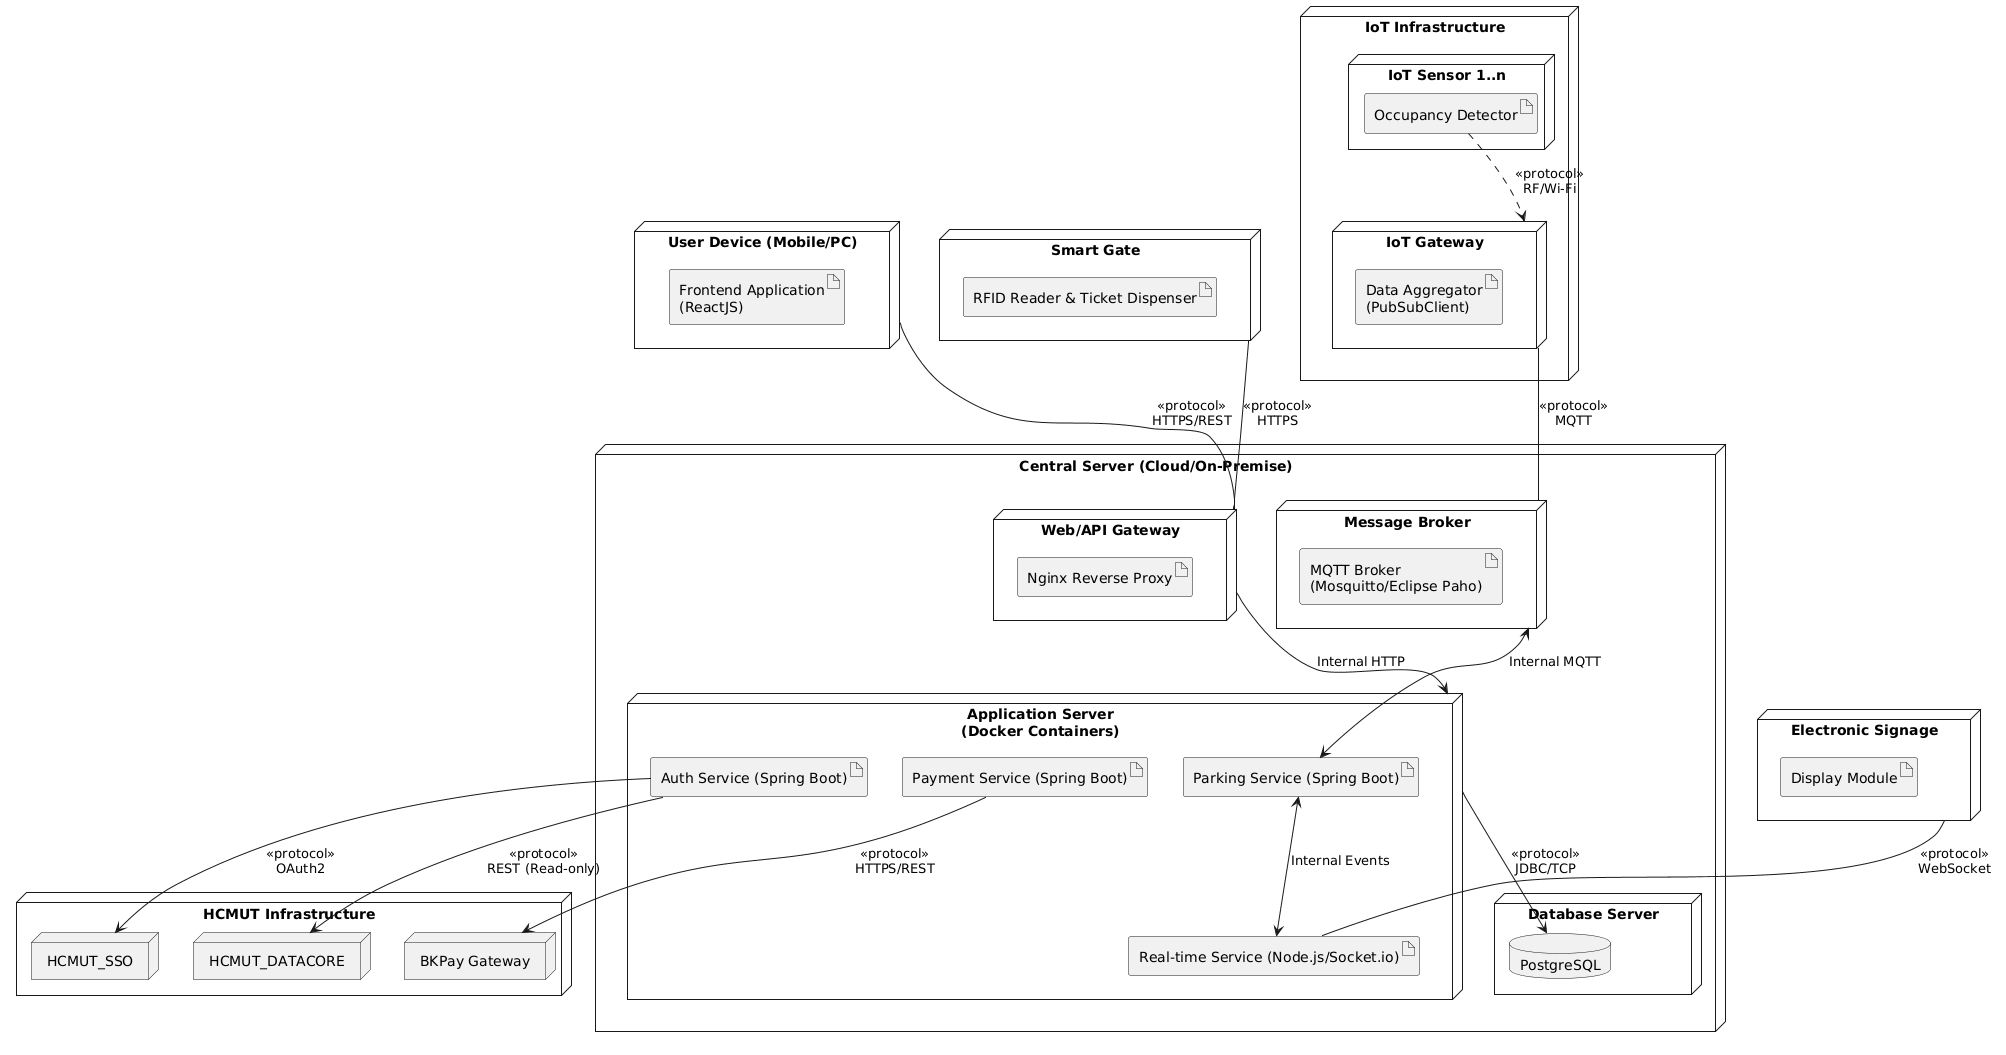
\includegraphics[width=0.9\linewidth]{pictures/deployment_diagram.png}
    \caption{Deployment Diagram của hệ thống IoT-SPMS}
    \label{fig:deployment_diagram}
\end{figure}